\documentclass[useAMS,usenatbib]{mnras}
% A Monthly Notices of the Royal Astronomical Society sample TeX file.
% The teX file has had all publication information removed and been left intentionally blank
\usepackage{graphicx}
\usepackage{float}
\usepackage{graphicx}
\usepackage{psfig}
\usepackage{amsfonts,amssymb,amsmath}
\usepackage{hyperref,color}
\usepackage{textcomp}
\usepackage[T1]{fontenc}
\usepackage{aecompl}
\usepackage{times}
\usepackage[colorinlistoftodos]{todonotes}
\usepackage{txfonts}
\usepackage[english]{babel}
\usepackage[utf8x]{inputenc}
\usepackage{amsmath}
\usepackage{graphicx}
\usepackage{caption}
\usepackage{subcaption}
\usepackage{siunitx}
%\usepackage{booktabs}

\usepackage[colorinlistoftodos]{todonotes}

%\usepackage[authoryear]{natbib}
%\graphicspath{ {images/} }

\def\aap{Astronomy \& Astrophysics}
\def\apj{The Astrophysical Journal}
\def\apjs{The Astrophysical Journal Supplement}
\def\mnras{Monthly Notices of the Royal Astronomical Society}
\def\pasp{Publications of the Astronomical Society of the Pacific}
%
\title{Estimating the probability of causal contact between
civilizations through MonteCarlo simulations}


% Group authors per affiliation:
\author[M. Lares et al.]
{M. Lares\thanks{E-mail: marcelo.lares@unc.edu.ar}\footnotemark[0] $^{1,2,3}$,
J. Funes $^{3, 4}$
\\
% institutions
$^{1}$Instituto de Astronom\'{\i}a Te\'orica y Experimental (CCT C\'ordoba, CONICET, UNC), Argentina.\\
$^{2}$Observatorio Astron\'omico de C\'ordoba, Universidad Nacional de C\'ordoba, Argentina.\\
$^{3}$Consejo Nacional de Investigaciones Cient\'{\i}ficas y
T\'ecnicas, Argentina.\\
$^{4}$Universidad Católica de Córdoba, Argentina
}
%
%\hypersetup{draft}
\begin{document}

\date{Accepted . Received ; in original form }

%\pagerange{\pageref{firstpage}--\pageref{lastpage}} \pubyear{2014}

 \maketitle

\label{firstpage}

\begin{abstract}
%
The abundance of intelligent civilizations in the galaxy is a
longstanding question, which is often conceptualized as the problem
of the lack of received communication of the Fermi paradox.
%
Most efforts on the estimation of a number of intelligent
civilizations are centered on the Drake equation, although 
its factors are affected by large uncertainties, and it lacks a
temporal nature.
%
Here we present numerical simulations of stochastic processes of
emergence of civilizations with communication capabilities, and
the causal contacts among them.
%
We analyze the rate of causal contacts as a function of the mean
number of civilizations and the mean lifetime span distribution.
%
Our results indicate that, given the large distances involved, in
   the odds to obtain a contact in a few years of monitoring, assuming a
   perfect detection rate, are very rare.
\end{abstract}
%
\begin{keywords}
keyword1, keyword2
\end{keywords}
%
%%%%%%%%%%%%%%%%%%%%%%%%%%%%%%%%%%%%%%%%%%%%%%%%%%%%%%%%%%%%%%%%%%%%%%%%%%%%%%%%%%%%
% Introduction
%%%%%%%%%%%%%%%%%%%%%%%%%%%%%%%%%%%%%%%%%%%%%%%%%%%%%%%%%%%%%%%%%%%%%%%%%%%%%%%%%%%%


\section{Motivations: Uncertainties and the non detection problem for
ETI contact}
%{{{

For citation purposes \citep{Lineweaver2004}
For citation purposes \citep{Forgan2011}
For citation purposes \citep{Rahvar2016}
For citation purposes \citep{Glade2011}
For citation purposes \citep{Dayal2016}
For citation purposes \citep{Gobat2016}
For citation purposes \citep{Prantzos2013}
For citation purposes \citep{Horvat2007}
For citation purposes \citep{Starling2013}
For citation purposes \citep{Barlow2012}
For citation purposes \citep{Tarter2009}
For citation purposes \citep{Forgan2017}
For citation purposes \citep{Forgan2013}
For citation purposes \citep{Wright2015}
For citation purposes \citep{Loeb2006}
For citation purposes \citep{Solomonides2016}
For citation purposes \citep{Fogg1987}
For citation purposes \citep{Anchordoqui2017}
For citation purposes \citep{Balb2018}
For citation purposes \citep{Forgan2010}
For citation purposes \citep{Forgan2008}
For citation purposes \citep{Forgan2016}
For citation purposes \citep{Haqq-Misra2017}
For citation purposes \citep{Forgan2015}
For citation purposes \citep{Gleiser2010}
For citation purposes \citep{cirkovic_temporal_2004}

For citation purposes \citep{cirkovic_temporal_2004}










A common approach to discuss the possible number of extraterrestrial
intelligent civilizations (ETI) has been the use of the Drake equation
\citep{}.

Uncertainties in the factors

Stochastic Drake equation and probabilistic approaches


Time:
The Impact of the Temporal Distribution of Communicating Civilizations on Their Detectability
Temporal dispersion of the emergence of intelligence: an inter-arrival time analysis
The spatiotemporal aspects of SETI
\citep{Fogg1987, Forgan2011, Balb2018}


Effort on considering the stochastic nature of the Drake equation
\citep{Glade2011}.


Simulation approach
New numerical determination of habitability in the Galaxy: the SETI connection
\citep{Forgan2008, Forgan2010}



Since the factors in the Drake equation are uncertain, we propose to
avoid the frequentist approach of this equation
and to explore a parameter space, where instead of computing a final
number, we provide a statistical distribution that gives conditional
probabilities.
%
The only fact that can be stated with certainty is that for the number
of years SETI projects have been working we have not received any
signal within the conditions stablished by SETI.



The discrete events method for simulating a stochastic process is an
approximation that allows to study the behaviour of complex
systems, by considering a sequence of well defined discrete events.
%
The simulation os carried out by following all the variables that
describe the system, that constitute the state of the system.
%
The evolution of the process, then, is described as a set of changes
in the state of the system.
%
In this context, an event produces a specific change in the state,
that can be triggered by random variables that encode the stochastic
nature of the physical phenomenon.
%
The process involves following the changes on the state of the system,
definig the initial and final states, defining a method that allows to
keep track of time progress, and maintaining a list of relevant
events.
%}}}



\section{Methods: accounting for causal contacts with 
discrete event simulation process}
%{{{

Some complex stochastic processes can be efficiently modeled with the
discrete--event (DE) simulation approach.
%
Simulations are suitable tools to analyze systems that evolve with
time and involve randomness.
%
In general, simulations require less assumptions and simplifications
than theoretical approaches, and can be applied to systems where 
a theoretical model can not be found.
%
A system described with the DE paradigm is characterized by a set of
actors and events, where actors interact causally through a series of
events on a time line and process these events in chronological order
\citep{ptolemaeus_book, chung_book, simulation_book}.
%
On the particular case of the difusion of signals of intelligence in
the Galaxy, the discrete events method can be performed taking into
account a small number of variables.
%
The temporal structure is defined by two distribution parameters that
represent the mean time interval that an intelligent civilization can
emit and receive signals, and the mean time interval between the
emergence of an intelligent comunicating civilization and the next one.
%
The spatial structure of the simulation is given by the size and shape
of the Galactic Habitable Zone and the maximum distance a signal can
travel to be detected.
%
The parameters for the temporal distributions also determine the
spatial properties.
%
For example, the density of active cetis in the Galaxy depend on these
two parameters.
%
Also, some hypothesis must be made in order to complete the
simulation, namely:

\begin{itemize}
   \item The capacity to emit signals and to receive signals ocurr at
      the same time.
   \item All CETIs use the same signal power, so that there is a
      maximum distance out to which it can be detected.
   \item The distribution of the appeareance of new CETIs
      is a stationary Poisson distribution.
   \item The distribution of duration of CETIs
      is a stationary exponential distribution.
   \item There is no a temporal window 
   \item The probability for the rise of a CETI is homogeneous
      over the GHZ.
   \item The message travels at light speed.
\end{itemize}

The exponential distribution of lifespan and waiting times is
justified by considering that the process of appeareance of life in
the galaxy is homogeneous and stationary.
%
This means that there is no preferred location within the GHZ for the
spontaneos appeareance of life, and that the emergence of a
civilization is independent of the existence of previous civilizations 
in the galaxy.
%
This is equivalent to proposing a Poisson process for the emergence of
CETIs, since there is a close relation between the number of events in
time or space and the waiting time or separation, respectively.
%
That is, these are two alternative approaches to describing the same
process, a Poisson distribution for the number of events implies an
exponential distribution for their sepations, and viceversa.
%
It should be emphasized that the exponential laws used in this work
are assumed, although instead of analyzing results from a particular
parameter chosen ad--hoc, we explore the hypothesis space and analyze
the impact of the values of these parameters on the results.
%


\subsection{Power laws vs. exponential laws}

The power law and exponential statistical distributions are among the
most common patterns found in natural phenomena.
%
For example, the distribution of the frecuency of words in many
languajes is known to follow a Zipf law (which is a power law).
%
Zipf law also describes population ranks of cities in various
countries, corporation sizes, income rankings, ranks of number of
people watching the same TV channel (Zipf's law entry on Wikipedia).
%
The magnitudes of earthquakes, hurricanes, volcanic eruptions and
floods; the sizes of meteorites or the losses caused by
business interruptions from accidents, are also well described by power
laws (Sornette 2006).
%
\itshape
Other studies have
documented power laws in stock market fluctuations,
sizes of computer files and word frequency in languages
(Mitzenmacher, 2004; Newman, 2005; Simkin \& Roy-
chowdhury, 2006).
In biology, power laws have been particularly impor-
tant in analysing connectivity patterns in metabolic
networks (Barabasi \& Albert, 1999; Ravasz et al., 2002)
and in the number of species observed per unit area in
ecology (Garcia Martin \& Goldenfeld, 2006).
(VER Frank, the common patterns of nature).
\slshape



Also, exponential laws arise when...




\subsection{Exploration of the parameter space}


Zipf law.

The adopted values for the GHZ are XX and XX \citep{Lineweaver2004}.

        

\begin{table}
\begin{tabular}{ccc}
\hline
   parameter & \multicolumn{2}{c}{adopted value}\hfill \\
\hline
   inner GHZ radius & \multicolumn{2}{c}{}\\
   outer GHZ radius & \multicolumn{2}{c}{}\\
\hline
   parameter & min & max \\
\hline
   D$_{max}$ & & \\
   $\tau_{a}$ & & \\
   $\tau_{N}$ & & \\
\hline
\end{tabular}
\caption{Adopted values for fixed and variable parameters in the
   simulation}
\label{T_parameters}
\end{table}

                


The fixed variables of the simulation are not explored:


\begin{itemize}
   \item Size of the GHZ
\end{itemize}


The variables that are explored with the simulation are:

\begin{itemize}
   \item Mean number of CETIs (Drake equation), or equivalently, the
      mean time between the awakening of two consecutive CETIs,
      $\tau_N$
   \item Mean lifetime of a CETI, $\tau_a$
   \item Maximum reach of CETI messages, $D_{max}$
\end{itemize}

The main variables that follow the evolution of the simulation are:

\begin{itemize}
   \item Position of stars.  Sampled randomly within the GHZ
   \item Time of the awakening of each CETI
   \item Time of the vanishing of each CETI
\end{itemize}

The variables that can be deduced from the previous ones are:

\begin{itemize}
   \item Number of CETIs in casual contact with at least another CETI
      at a given time.
   \item Number of CETIs as a function of time
   \item Number of CETIs that receive a message at least one time
   \item Number of CETIs that receive a message at least one time and
      successfully deliver an answer.
   \item Number distribution of waiting time to receive a message
\end{itemize}


%========================================================================
%========================================================================
%========================================================================
                   

\begin{figure}
   \centering
   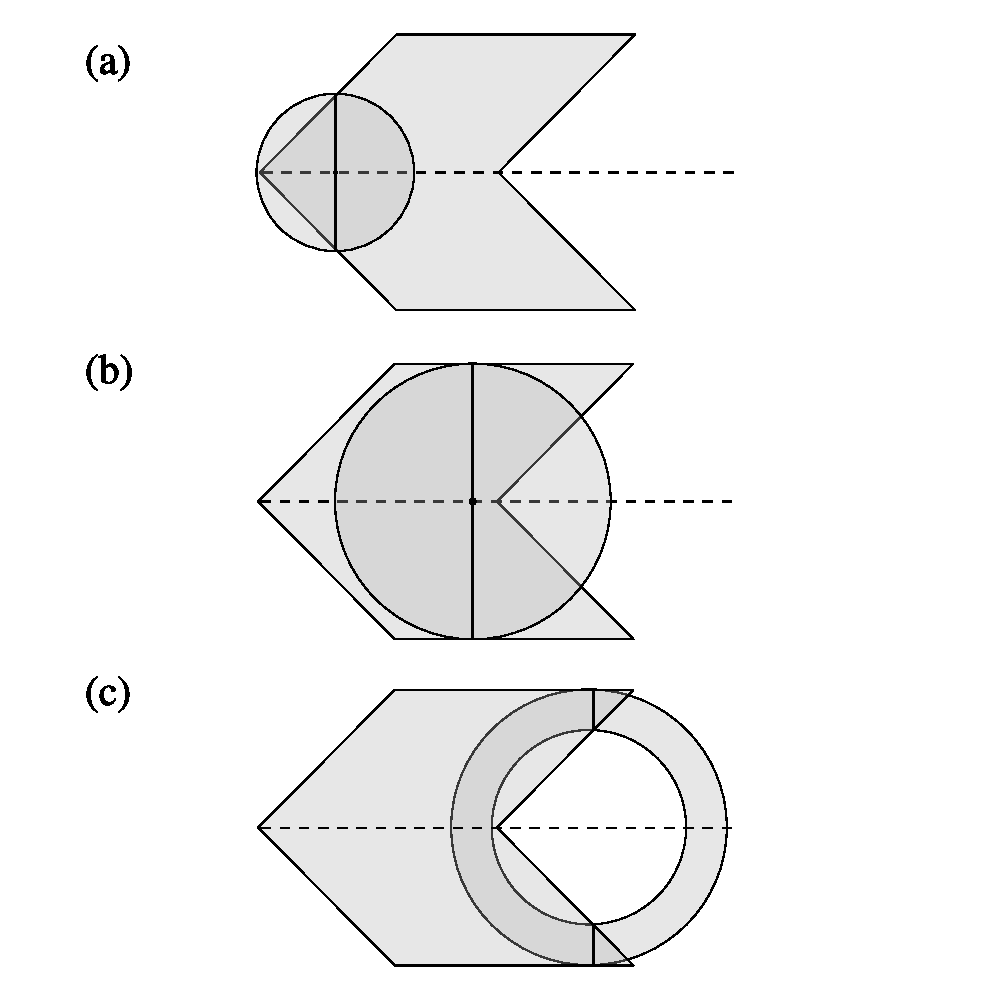
\includegraphics[width=0.5\textwidth]{growingsphere.pdf}
   \caption{Schematic representation of the growing communicating
   sphere, over the space--time diagrams.  In (a) the sphere is
   growing as the surface of first contact has not reached the maximum
   distance.  In (b) it has reached the maximum distance, so that it
   remains at the same size.  After a Doomsday event, the signals can
   still be observed, but the surface of last contact grows }
   \label{F_sphere}
\end{figure}

  
\begin{figure}
   \centering
   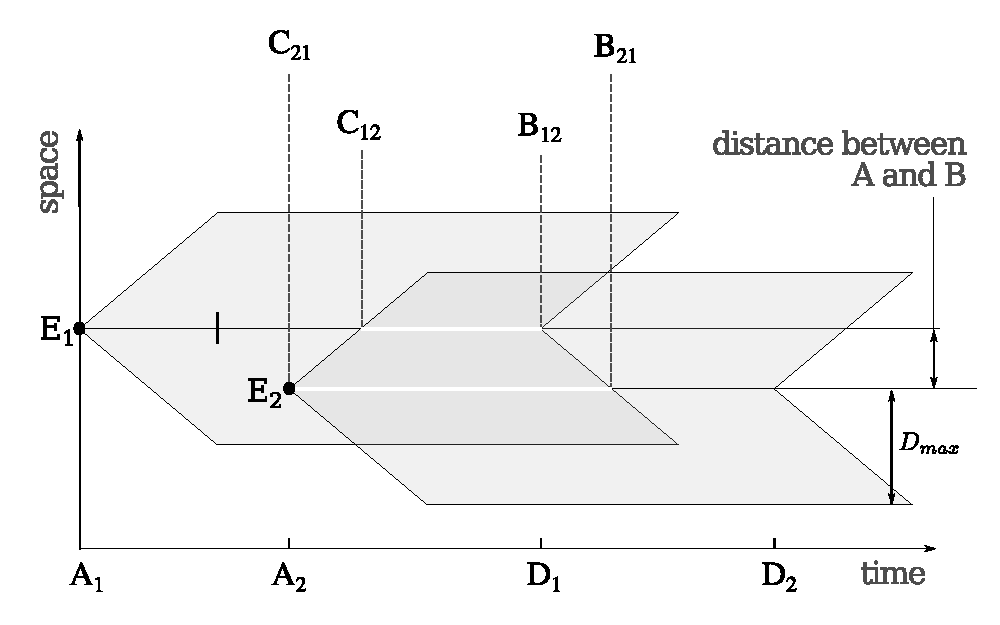
\includegraphics[width=0.5\textwidth]{abcd.pdf}
   \caption{Schematic representation of two emitters, $E_1$ and $E_2$,
   that reach each other at different times.  The time span for $E_i$
   is $(A_i, D_i)$, for $i=\{1,2\}$.  Emitter $i$ can listen to
   emitter $j$ between $C_{ij}$ and $B_{ij}$.
   The type and length of causal contact in both directions depend on
   the distance and time lag between the awakening events, the maximum
   distance that a signal can reach and the time period in which each
   emitter is active.}
   \label{F_abcd}
\end{figure}
                     

Possible hypothesis improvements are:

\begin{itemize}
   \item Dmax is different for different CETIs.  For example a power
      law where powerfull emmisions are rare and weak emssions are
      common.
   \item The probability of the rising of a new CETI vary within the
      GHZ.
   \item Correction by coverage ratio in the detection and by
      targetting ratio in the emission.
   \item Spiritual factor.  Explore the role of the S factor: message
      contents, influence on the lifespan of a CETI that receives a
      message, mean lifespan of a CETI that emits a message.
\end{itemize}


\subsection{Model for CETIs}


Since the method is based on events, the first step is to define an
architecture of events, the relationships between them and how events
trigger changes on the state of the system.
%
We consider a simulated system that represents the galactic habitable
zone (GHZ).
%
On a first approach, the GHZ is a 2-dimensional annular region.
%
This simple model does not take into accont the variations in stellar
density given by the spiral structure.
%
Although there are several possible approaches, we chose to follow the
evolution of the system according to the following events:


\begin{enumerate}
   \item[(A)] A new CETI appears (Awakening)
   \item[(D)] An old CETI dissappears (Doomsday)
   \item[(C)] A new causal contact is stablished (Contact)
   \item[(B)] An existing causal contact is interrupted (Blackout)
\end{enumerate}


The event of type B is produced when one of the two CETIs halts in its
capability of emmiting and receiving signals.













%======================================================================
%======================================================================
%======================================================================


The system is updated each time an event is produced.  The time marks
for each event (A and D for each CETI and C and B for each causal
contact) are stored as a result of the simulation.
%
Also, the list of active CETIs is obtained as a function of time.

Some fixed variables must be set in order to carry out the simulation,
namely:

\begin{itemize}
   \item Size of the Galactic Habitable Zone.  Radial symetry is
      assumed, so that the GHZ is determined by two radii, the inner
      radius (GHZ\_inner) and the outer radius (GHZ\_outer).  They are
      measured in light years, with the aim to maintain y single and
      comprehensive unit for both space and time coordinates.
   \item Mean lifetime of a CETI
   \item Mean waiting time for the appeareance of another CETI
   \item Maximum distance a message can be detected
\end{itemize}


%Variables en el programa
%\begin{itemize}
%   \item Nact: Número de CETIs activas
%   \item Nsee: Número de contactos por cada CETI
%   \item Nccc: CETIs en contacto causal. Notar que una CETI puede tener múltiples
%contactos de otras CETIs. Para cada una de ellas, guardar:
%   \item ID: ID de la CETI emisora
%   \item ID: ID de la CETI receptora
%   \item t\_hola: tiempo del primer contacto
%   \item t\_chau: tiempo del último contacto
%\end{itemize}
%
%
%Caso 1: aparece una nueva CETI
%Modificaciones al estado del sistema:
%\begin{itemize}
%   \item Agregar la CETI “A” a la lista de CETIs activas
%   \item Sortear la duración de la actividad de comunicación de la CETI “A”
%   \item Sortear el intervalo de tiempo hasta la aparición de la próxima CETI:
%t\_WakeUp\_next
%   \item Agregar la CETI “A” al árbol
%   \item Identificar todas las CETIs que están a menos de D max de la nueva CETI, y
%actualizar la lista de tiempos
%\end{itemize}
%
%Caso 2: desaparece una CETI
%Modificaciones al estado del sistema:
%\begin{itemize}
%   \item Eliminar la CETI a la lista de CETIs activas
%\end{itemize}
%
%
%Caso 3: una nueva CETI entra en contacto causal
%Modificaciones al estado del sistema:
%\begin{itemize}
%   \item Agregar la CETI B a la lista de contactos de la CETI A
%\end{itemize}
%


%}}}


\section{Results: exploring the parameter space}
%{{{

As the result of the simulation, several quantities are obtained.

Direct quantities are:

\begin{itemize}
   \item ID of emitting CETI
   \item ID of emitting (receiving) CETI 
   \item x position in the galaxy
   \item y position in the galaxy
   \item time of Awakening (Contact)
   \item time of Doomsday  (Blackout)
\end{itemize}

This structure is always for the A-D cycle of each emitting CETI,
and repeats for each contact (C-B).
%
We define the following quantities: age is the time elapsed from A to a
given time, ceti\_e is the CETI emitting signals (emiter), ceti\_r is
the CETI receiving signals (receiver), ceti\_c is the ceti that listen
at least another ceti (citizen) and ceti\_h is the CETI ceti that is
lestened by at least another CETI.

Then, several derived quantities can be obtained:

\begin{itemize}
   \item time span of a ceti listening another
   \item time span of a ceti being listened by another
   \item duration of two-way communication channels
   \item waiting time until the first contact
   \item waiting time until the next contact
   \item fraction of awaken time a ceti is listening at least another ceti 
   \item age of contacted cetis\_e at first C
   \item distribution of time to wait until next C
   \item fraction of cetis where the first contact is given at the A       
   \item distribution of the number of contacts for each ceti         
   \item distribution of the maximum number of contacts for each ceti 
   \item distribution of the number of contacts as a function of age  
   \item number of contacts as a function of time in the galaxy       
   \item rate of cetis that succeed in contact                        
   \item fraction of contacts that admit a response                   
   \item distribution of distances between contacted cetis 
   \item relation between distance to ceti and time of double communication 
   \item relation between distance to ceti and age of contacted ceti
   \item relation between the age of a ceti and the maximum number of contacted cetis before D
   \item relation between lifespan of a ceti and max number of contacts
   \item distribution in the galaxy of cetis that reach contact
\end{itemize}


All these quantities can be analyzed as a function of the simulation
parameters.

%}}}


\subsection{Duration of contacts}
%{{{

%}}}


\subsection{Waiting time for a first contact}
%{{{

In this section we analyze the distribution of the waiting times for
a first contact.
%
Such distribution can be considered to compute the probability of
reaching a first contact within the first XX years.


%}}}


\subsection{Reciprocal communication}
%{{{

%}}}


\subsection{Location within the Galaxy}
%{{{

%}}}


\begin{figure*}
   \centering
   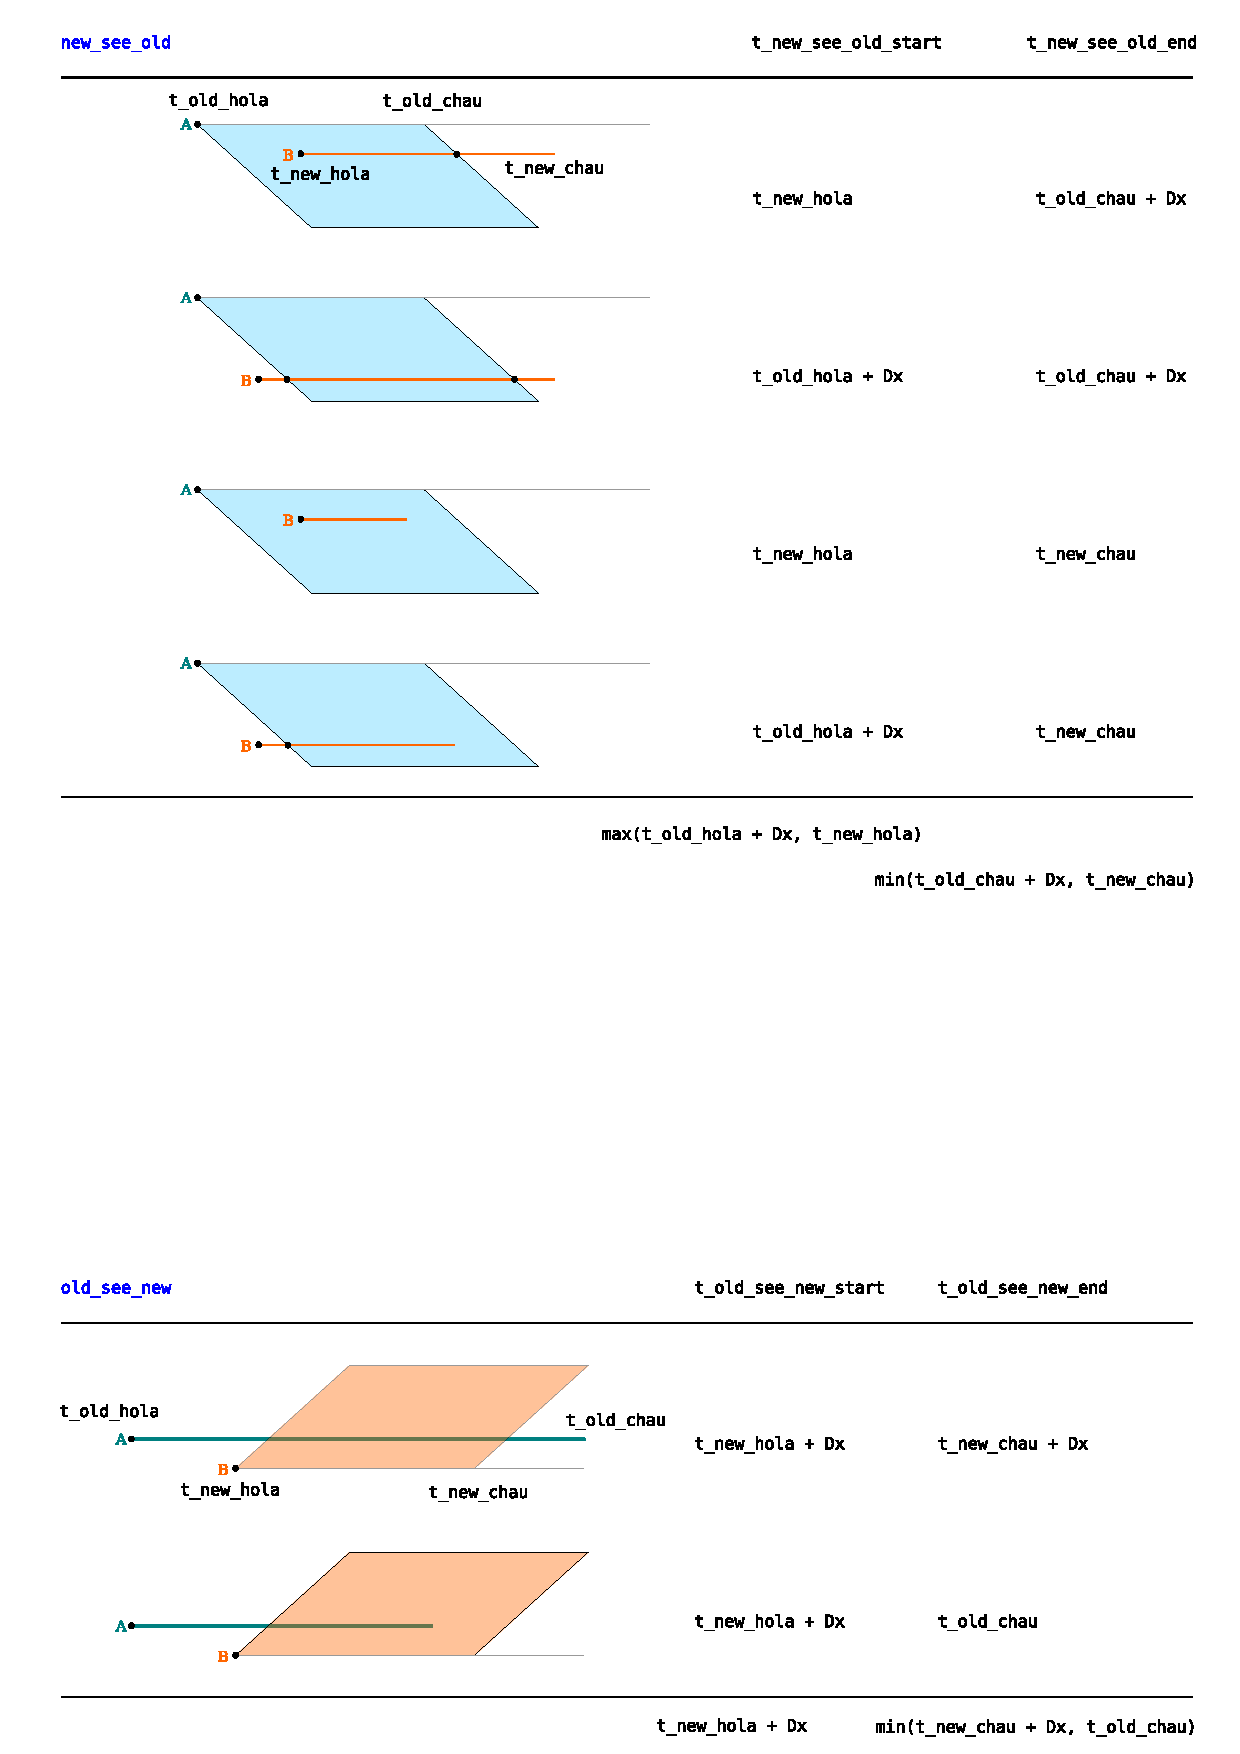
\includegraphics[width=\textwidth]{Messages_01.pdf}
   \caption{Schematic representation of the possible cases in which a
   ceti A can be in causal contact with a ceti B which appears later.
   The duration of the causal contact in one direction depends on
   several factors, mainly $\Delta t_A$, $\Delta t_C$, and $\Delta X$.}
   \label{F_messages}
\end{figure*}
 

\section{Discusion}
%{{{

Possible implications of the results:

\begin{itemize}
   \item Analysis of the communication method: isotropic, colimated,
      serendipitous
   \item Nature of the message carrier: electromagnetic or another
   \item Effects of alignments
   \item energetic markers
   \item Spiritual markers
   \item Use of stars as sources or amplifiers
\end{itemize}


Under the hypotheses of our experiments, we conclude that
a causal contact is extremely unlikely unless the Galaxy is heavily
populated by intelligent civilizations.
%
Even so, we must consider that in order to stablish a contact between
any two entities, a minimum degree of compatibility must be
accomplished without any previous agreement, 
making the posibility of a contact with a message that
could be deciphered highly rare.
 
%}}}

\bibliographystyle{mn2e}
\bibliography{biblio_seti}
\end{document}
